\section{Experimental Results}\label{sec:4}%
\newcommand{\car}[1]{\emph{#1}}%

The drivers were developed in C++ and testing in TORCS\footnote{\url{http://sourceforge.net/projects/torcs/}} (v1.3.6) and SCR\footnote{\url{http://sourceforge.net/projects/cig/files/SCR\%20Championship/Server\%20Linux/}} (v2.1), since they provide an advanced simulation environment which provides complex situations, and enable objective metrics for direct comparison to exiting results. The standard the car model for racing in SCR is \car{car1-trb1}~\cite{SCR}.

\gnramos{revisado - GA foi aplicado a todos os 22/17 parametros? yes}

Once the FSMDriver models had been defined, a genetic algorithm was applied to each, aiming to improve their performances by changing their control parameters' values. During this stage, the learning module was disabled in FSMDriver3 in order to not interfere with the learning. Then drivers' performance is evaluated by racing them in selected tracks, emulating the qualifying stage of SCR. Also similar to the competition, before each qualifying race a warm-up stage is held in order for the controllers to adapt themselves to the track. In this stage, two versions of the 3-state FSM controllers were tested to analyze the effects of the learning module, the FSMDriver3+ with the the module enabled, and FSMDriver3, with it disabled. This lasts for 5 laps, conforming to the stipulated 2015 Championship rules\footnote{\url{http://cs.adelaide.edu.au/~optlog/SCR2015/}}.

\gnramos{revisado, formula colocada nos comentarios, ponderar a sua necessidade - qual das formulas?}
% G = 267,43*ln(P) - 293,21 (G = generations, N = population size)
The Genetic Algorithm used standard configurations from literature, the population size was arbitrarily set as 30~\cite{RATES}, which leads to 616 generations for a moderate problem complexity in which the optimal population size was coded as bitstrings~\cite{218485}. Selection is done through elitism by keeping the best 4 individuals from a generation unchanged, and the other 26 are generated from the best 10 individuals' reproduction~\cite{ELITISM}. This step is done by randomly choosing a pair from the top 10 that are cloned with a 5\% chance or generate a pair of offspring with a 95\% probability~\cite{RATES}. These offspring are produced through crossover by partitioning the parents' bitstrings at a random position and swapping them. Finally, mutation (a simple bit flip) is applied to every bit in every individual of these 26 with a 1\% probability~\cite{RATES}.

\newcommand{\profile}[1]{\emph{#1 driver}}%
Since it is unknown which tracks will be used during the SCR Championship, a more general and versatile controller is desirable and, thus, the controllers were evolved considering their performance in several tracks types. Three basic driver profiles were desired: a \profile{road}, which would perform well in road tracks, a \profile{dirt}~ for dirt roads and a \profile{mixed}, which should perform well in both types.

\newcommand{\track}[1]{\emph{#1}}%
For the \profile{road} profile, four road tracks were selected from the standard TORCS distribution list to compose the training set in the evolution process. The tracks were arbitrarily selected for certain features, which might lead to better drivers: \track{Spring}, the longest track available; \track{Wheel 2}, with many sharp curves; \track{E-Track 3}, a fast track with sharp curves; and \track{Forza}, a fast circuit with smoother curves.

Analogously, four dirt tracks were selected for evolving a \profile{dirt profile}: \track{Dirt 2}, \track{Dirt 6}, \track{Mixed 1}, and \track{Mixed 2}, which present variations of high speed and curve styles. For the \profile{mixed}, two of each were selected: \track{Spring}, \track{Wheel 2}, \track{Dirt 2}, and \track{Mixed 1}.

\gnramos{inserir exemplo de resultados de evolucao, talvez uma tabela mostrando os tempos em relacao a bots}

The best solutions evolved for each profile where then evaluated in a set of six tracks, different from the ones used before, which present distinct typed, speeds, and curve features for better analysis. These tracks, also available on the standard TORCS set, were used in previous SCR Championships~\cite{AUTOPIA2009}. They are two road tracks: \track{Street 1} and \track{CG Speedway 1}; one oval track: \track{D-Speedway}; and three dirt tracks: \track{Dirt 1}, \track{Dirt 3}, and \track{Dirt 4}.

\begin{figure*}
\centering
\begin{subfigure}[b]{0.2\textwidth}
       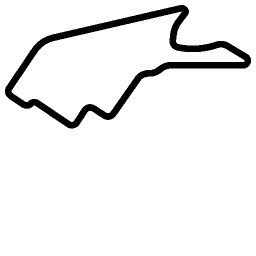
\includegraphics[width=\textwidth]{img/tracks/Street1}
       \caption{Street1}
   \end{subfigure}
\begin{subfigure}[b]{0.2\textwidth}
       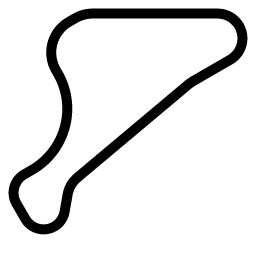
\includegraphics[width=\textwidth]{img/tracks/CG-Speedway}
       \caption{CG Speedway 1}
   \end{subfigure}
\begin{subfigure}[b]{0.2\textwidth}
       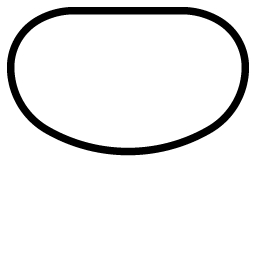
\includegraphics[width=\textwidth]{img/tracks/D-Speedway}
       \caption{D-Speedway}
   \end{subfigure}

\begin{subfigure}[b]{0.2\textwidth}
       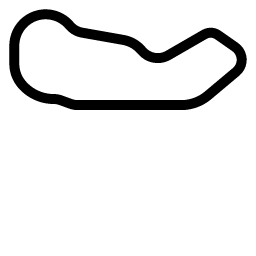
\includegraphics[width=\textwidth]{img/tracks/Dirt1}
       \caption{Dirt 1}
   \end{subfigure}
\begin{subfigure}[b]{0.2\textwidth}
       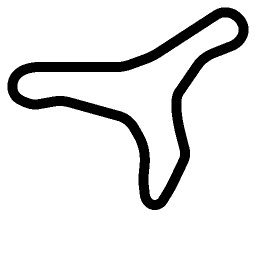
\includegraphics[width=\textwidth]{img/tracks/Dirt3}
       \caption{Dirt 3}
   \end{subfigure}
\begin{subfigure}[b]{0.2\textwidth}
       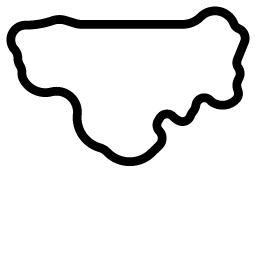
\includegraphics[width=\textwidth]{img/tracks/Dirt4}
       \caption{Dirt 4}
   \end{subfigure}
   \caption{Test tracks, road tracks (top left and middle), oval (top right), and dirt tracks (bottom)~\protect\cite{TORCS}.}\label{fig:tracks}
\end{figure*}

\subsection{Single Race Results}

\gnramos{revisado - fsmdriver 5 na CG é isso mesmo? resultado corrigido}
\begin{table*}
% \renewcommand{\arraystretch}{1.3}
\caption{Distance covered (in meters) racing alone for 10.000 game ticks}\label{tbl:ticks}
\centering
\begin{tabular}{| c | c || c | c | c | c | c | c |}
\cline{3-8}
\multicolumn{2}{ c | }{} & \multicolumn{6}{ c |}{\bfseries Track} \\\hline
\multicolumn{2}{| c ||}{\bfseries Driver} & \bfseries Street 1 & \bfseries CG-speedway & \bfseries D-speedway & \bfseries Dirt 1 & \bfseries Dirt 3 & \bfseries Dirt 4 \\\hline\hline
\multirow{3}{*}{FSMDriver5}
& road  & 3822.76 & 4114.66 & 3427.11 & 2145.49 & 2205.97 & 3260.19 \\\cline{2-8}
& dirt  & 1267.83 & 2057.47 & 2936.82 & 1072.92 & 2205.82 & 3260.33 \\\cline{2-8}
& mixed & 3822.99 & 4114.80 & 3427.06 & 2145.75 & 2205.83 & 3260.31 \\\hline\hline
\multirow{3}{*}{FSMDriver3}
& road  & \textbf{7925.60} & 8745.49 & 13196.50 & 3978.01 & 3451.26 & 6757.83 \\\cline{2-8}
& dirt  & 5103.41          & 5093.82 &  8589.13 & 3525.84 & 4905.58 & 5590.78 \\\cline{2-8}
& mixed & 5864.48          & 8714.58 & 11694.60 & 5052.38 & 4920.32 & 3797.83 \\\hline\hline
\multirow{3}{*}{FSMDriver3+}
& road  & 7532.93 & 8804.73 & 10720.20 & 3678.89          & 5199.46 & 3193.44 \\\cline{2-8}
& dirt  & 4738.76 & 5102.92 &  8197.55 & 3525.84          & 4214.30 & 5057.18 \\\cline{2-8}
& mixed & 6780.43 & 8089.41 & 10943.10 & \textbf{5752.90} & \textbf{5824.93} & \textbf{5614.62} \\\hline\hline
\multicolumn{2}{| c ||}{AUTOPIA~\cite{AUTOPIA2009}} & 7091.8 & \textbf{8970.4} & \textbf{15612.3} & * & * & * \\\hline
\end{tabular}
\end{table*}

Table~\ref{tbl:ticks} presents the distance covered results for these tests for each FSMDriver model and profile. The fitness function in this case is the sum of distances covered in all tracks, considering 10.000 game ticks per track, as per the SCR rules, so higher values are desirable. The table also includes, for direct comparison with the current state of the art, results for AUTOPIA in three of the same tracks for the same 10.000 game ticks metric, as presented in~\cite{AUTOPIA2009}. The `*' symbol indicates that the driver does not have data available for the track.

Considering the 5-states FSMDriver in road/oval tracks, it is clear that the road and mixed profiles have better results than dirt, as expected. However, in \track{CG Speedway 1} they are practically the same. \gnramos{por que?} Looking at the results for dirt tracks, all profiles have similar performances except for the dirt profile in \track{Dirt 1}. \gnramos{por que?}

Considering the 3-states FSMDriver in road/oval tracks, it is also clear that the road and mixed profiles have better results than dirt, as was expected. Looking at the results for dirt tracks, the mixed profile's performance was significantly better than the others. FSMDrivers evolved in dirt tracks tend to drive slower to avoid leaving the track limits while evolution in road tracks leads to faster racers which may lose time off track. The combination of both tracks in the metric leads to drivers that compromise in both approaches, being about 5-10\% slower than the road profile in road tracks, and about 5-15\% faster in dirt tracks,a more general driver as hypothesized. It is also better than the dirt profile on all accounts.

Comparing the results with AUTOPIA, the road FSMDriver3 was about 11.7\% better in \track{Street 1}. By itself this does not imply that FSMDriver3 is a better approach, specially since AUTOPIA had better results in two of the three tracks compared, it still is an impressive result for this simpler approach to driving.

In order to learn more about FSMDriver's potential, a new set of tests using the distance raced in 10 laps as metric was done, and the results are shown in Table~\ref{tbl:time}. The values represent the time needed to complete the laps, so lower values are desirable, the `\textdagger'~symbol indicates that the driver does not complete the 10 laps required, and the `*' symbol indicates that the driver does not have data available for the track. Again results for AUTOPIA in three of the same tracks for the same 10 laps metric, as presented in~\cite{AUTOPIA} are shown for comparison.

Table~\ref{tbl:time} also includes results for the robot \emph{Berniw Hist4}, provided in with the TORCS distribution. This was not included in the previous tests because TORCS only allows a race with the available robots to run for a given amount of laps (not game ticks). This robot has intermediate performance, and was arbitrarily chosen from other robots to provide insights on the controllers performance compared to a robot's and to AUTOPIA, as presented in ~\cite{AUTOPIA}. Direct comparison is not possible because \emph{Berniw Hist4} does not the standard car \car{car1-trb1}, it uses the \car{TZ2}.

\begin{table*}[t]
	% \renewcommand{\arraystretch}{1.3}
\caption{Time elapsed (in seconds) racing alone for 10 laps}\label{tbl:time}
\centering
\begin{tabular}{| c | c || c | c | c | c | c | c |}
	\cline{3-8}
\multicolumn{2}{ c | }{} & \multicolumn{6}{ c |}{\bfseries Track} \\\hline
\multicolumn{2}{| c ||}{\bfseries Driver} & \bfseries Street 1 & \bfseries CG-speedway & \bfseries D-speedway & \bfseries Dirt 1 & \bfseries Dirt 3 & \bfseries Dirt 4 \\\hline\hline
\multirow{3}{*}{FSMDriver5}
& road  & \textdagger & 816.6       & \textdagger & \textdagger & \textdagger & \textdagger \\\cline{2-8}
& dirt  & \textdagger & \textdagger & \textdagger & \textdagger & \textdagger & \textdagger \\\cline{2-8}
& mixed & \textdagger & \textdagger & \textdagger & \textdagger & \textdagger & \textdagger \\\hline\hline
\multirow{3}{*}{FSMDriver3}
& road  & \textbf{1086.28} & \textbf{483.17} & \textbf{607.35} & \textdagger & 1150.09 & \textdagger \\\cline{2-8}
& dirt  & \textdagger      & 1274.81         & 840.02          & 597.33      & 1045.62 & 1307.52  \\\cline{2-8}
& mixed & 1096.95          & 510.86          & 612.00          & 408.57      & 811.96 & 2157.95 \\\hline\hline
\multirow{3}{*}{FSMDriver3+}
& road  & 1225.24 & 484.58  & 709.74 & \textdagger & 1108.48 & \textdagger \\\cline{2-8}
& dirt  & 1658.47 & 1291.31 & 915.86 & 597.33 & 1055.21 & 1360.71 \\\cline{2-8}
& mixed & 1208.84 & 534.87  & 646.68 & 384.93 & 939.93 & 1930.19 \\\hline\hline
\multicolumn{2}{| c ||}{Berniw Hist4} & 1143.77 & 605.76 & 656.24 & 460.95 & 872.97 & 1127.45 \\\hline\hline
\multicolumn{2}{| c ||}{AUTOPIA~\cite{AUTOPIA}}  & * & * & * & \textbf{339.3} & \textbf{742.4} & \textbf{796.5} \\\hline
\end{tabular}
\end{table*}

Looking at results for FSMDriver5, only the road profile completed 10 laps in \track{CG Speedway 1}, all other instances had excessive damage. FSMDriver3, on the other hand, completed all track in at least 2 configurations. Considering road tracks, the road profile had better performance in two of the three tracks, and the dirt profile did not complete one but was significantly slower in two of the tracks. Considering the Dirt tracks, again the mixed profile's performance was significantly better than the others.

Considering the robot \emph{Berniw Hist4}, it can be seen that FSMDriver3 is a slightly better driver, despite the ``handicap'' of using SCR's interface for driving and not having access to additional information from the simulator (such as track layout). This means that the proposed model has quickly achieved an intermediate level performance in TORCS. AUTOPIA's results are around 12\%-35\% better than FSMDriver's best results, implying that its configuration is better suited for longer races.

This is likely due to lack of endurance, resulting from careless driving. Since dirt profile tends to drive slower, it drives farther on this longer test.





% \subsection{Analysis} \label{subsec:Analysis}

%	The overall comparison between the two approaches presented favored the Three-State FSM, on account of the considerably superior results it produced in all the tracks tested. The Five-State FSM presents a very complex transition function that takes into account the variance of the sensorial input to decide if the car is in a straight line, approaching a turn or in a turn. On the other hand, the Three-State FSM has only a single state for handling normal driving situations and it is very easy to say if the controller is inside or outside the track only by checking the track sensor. By having multiple states acting inside the track the Five-State FSM leads to a struggle in defining the boundaries of a curve, the characteristics of an approaching curve and how those situations are different from a straight line. Mismatching emergent from the transiction function would often cause the car to leave the track. It seemed that a single state for handling those situations ended in more accurate behavior on account of having no dependence from an external function.

%	Besides the difficulty in deciding on which state should be triggred. There is the complexity related to defining the behavior for each state. The steering control in the straight line was too smooth and sometimes depending on how the car left a curve it was not capable of correcting the trajectory and could led to those exception situations. However if the same control was too abrupt like the curve's one it would also led to exception situations due to excessive steer. These and other problems emphasized the need of a unified state for dealing with those situations.

%	This contrast in behavior is then interpreted to be the reason of the overwhelming difference in performance, the complexity of the transition function, which supports the initial hypothesis of the evaluation. Due to this attribute, the Five-State FSM undergoes a lot of damage in its car, which can be noted in Table~\ref{tbl:time raced} where all the ``\textdagger'' symbols represent individuals that did not finish the race for the reason of reaching the maximum damage permitted.

%	Because the Three-State FSM demonstrated better results than the other approach proposed, it was elected to be subject of analysis on the evaluation process. As expected, the controller evolved only on Road Tracks was the fastest one. These tracks provide an environment susceptible to high speeds, since its curves are smoother and the friction experienced by the car is higher than the ones from Dirt Tracks. These factors, when combined, allow the controller to race without having to steer too abruptly and to brake without losing control while racing in Road Tracks. Consequently, as the friction increases, steering becomes more accurate in road tracks, practically eliminating critical skidding. Therefore, the result from this end of the evolution process was an aggressive driver with high base-speed.

%	Dirt Tracks provide a more difficult environment for the pilot to fit in. Sudden braking in tracks of this type often results in unwanted behavior, skidding is noticeably more common then. The driver evolved in this end of the evolution process tends to drive in a low speed so it can keep itself inside the boundaries of the track. Speed driving results in higher damage outcomes and even in the total loss of the car in critical situations. The result obtained was a very careful driver with a low base-speed, and an early brake policy - the car starting to brake far before the turn. This passive driving pattern obtained the smallest distance covered both for the Three-State and the Five-State FSMs.

%	The driver evolved in a mixed set of tracks combines characteristics from both of them. It drives in a reasonable speed comparing to the first one, but also has the preventive brake policy from the second one. This last end of the evolution process achieved better results than the Dirt evolved behavior in all the tracks tested and outperformed the road-evolved one in every single dirt track. From this information gathered, it was inferred that the controller evolved in mixed tracks tries to reach higher speeds even though this means leaving the track in some turns, mostly because the time spent trying to get back to the racing lane is compensated by the speed of the car. The aggressive behavior inherited from the road-evolved end of the evolution makes this latest controller receive ample damage when leaving the track, and also causes it to hit walls, which resulted in the premature ending of some of the tested races, due to reaching the maximum acceptable damage.

% \subsubsection{Comparing the Three-State FSM to AUTOPIA} \label{subsubsec:CompAUTOPIA}

%	Once the Three-State FSM was demonstrated to be more suitable to competitive environments due to its superior performance regarding the Five-State FSM, it was compared to the renowned controller AUTOPIA. Using the distance covered after racing alone in Road Tracks for 10 000 game tics as metric, the Three-State FSMs evolved in Road Tracks and in mixed tracks were able to overcome AUTOPIA in 1 of the 3 tracks tested, as displayed in the bold values in Table~\ref{tbl:dist covered}. The road-evolved Three-State FSM was the controller that got closer to this State of the Art approach using the ``distance raced'', which comes to endorse the assumption of it being a competitive proposal.

%	However, while racing alone for 10 laps and computing the time elapsed as metric, AUTOPIA outperformed every controller proposed, just as can be seen in Table~\ref{tbl:time raced}. Even though the Three-State controller with Road evolved parameters outperformed AUTOPIA in the first 10 000 tics it was not capable of maintaining the advantage in longer races. The road evolved pilot presents a more aggressive behavior even though it means taking more damage it has a gain in performance for the early stages of the race. Although when racing for more than a couple laps the controller becomes more careful after each lap reducing it speed to maintain itself inside the track.

%	The graphical analysis was quite useful at this point. It revealed that AUTOPIA's brake, acceleration and recovery policies are robuster than the ones presented in this papper. AUTOPIA barely leaves and track and when it does a fast recovering behavior is performed  resulting in small losses in performance. It also has a better stability control which can be observerd moslty in Dirt tracks, where the car is more susceptible to splip and skidding.

%	The online learning module plays a crucial role in the overall controller's performance as it prevents unwanted situations to repeat, for example leaving the track. Although this strong dependence might result in performance loss as the controller will gradually reduces it speed after each lap in those points where it leaves the track. More accurate actuators control may reduce the dependence of this module and therefore improves performance.

%	These results can be used to infer that the Five-State and the Three-State FSMs have a great deal of improvement to achieve when it comes to endurance. The Five-State FSM received total loss and did not complete almost every test performed, ending only one race using this metric. The Three-State FSM, on the other hand, completed practically all the tracks, but did not surpass AUTOPIA in either of them. In order to enhance the endurance feature in the controllers proposed, more robust behavior concerning situations in which the car might crash must be taken into account.


\subsection{Analysis}
Further comparing both FSMDrivers, it is clear that different profiles lead to different performances on the tracks for FSMDriver3, but such effect is not as pronounced in FSMDriver5. A more detailed analysis shows that FSMDriver5 has issues handling transitions in \racing~behavior. The issue seems to be that the parameters \gnramos{???} in the transition function that define the current stated are very susceptible to the inputs, resulting in several changes in the states which greatly impacts the evolution of the states' parameters and, consequently, of those in the function.

This leads to two possibilities, the first being that the specified settings for evolving FSMDriver5 were not adequate, perhaps allowing more generations or individuals would lead to better results. More likely, the 5-state model's implementation is overly complex, specially considering the influence of the transition function's parameter \gnramos{parametros??} on how the states evolve, which could imply that a different strategy should be pursued.
